\documentclass{article}
\usepackage{lingmacros}
\usepackage[danish]{babel}
\usepackage{enumitem}
\usepackage{lmodern}
\usepackage[utf8]{inputenc}
\usepackage[T1]{fontenc}
\usepackage{color}
\usepackage{amssymb}
\usepackage{listings}
\usepackage{listingsutf8}
\usepackage{color} %red, green, blue, yellow, cyan, magenta, black, white
\definecolor{mygreen}{RGB}{28,172,0} % color values Red, Green, Blue
\definecolor{mylilas}{RGB}{170,55,241}
\lstset{literate=
  {æ}{{\ae}}{1} 
  {å}{{\aa}}{1} 
  {ø}{{\o}}{1} }
\usepackage{graphicx}
\usepackage[export]{adjustbox}
\usepackage{fullpage}
\lstset{basicstyle=\ttfamily,breaklines=true}
% \lstset{framextopmargin=50pt,frame=bottomline}
\lstset{
  % numbers=left, 
  % numberstyle=\small, 
  % numbersep=8pt, 
  frame = single, 
  language=Pascal, 
  framexleftmargin=15pt}
\usepackage[T1]{fontenc}
\usepackage[hidelinks]{hyperref}
% \usepackage{maplestd2e}
\usepackage{tree-dvips}
% \usepackage{biblatex}
% \usepackage[style=verbose,backend=bibtex]{biblatex}
% \bibliography{oeve1dsb.bib}
% \usepackage{sagetex}
\usepackage{amsmath}
% \usepackage{newpxtext,newpxmath}
\usepackage{courier}
\linespread{1.5}
\makeatletter
\renewcommand*\env@matrix[1][*\c@MaxMatrixCols c]{%
  \hskip -\arraycolsep
  \let\@ifnextchar\new@ifnextchar
  \array{#1}}
\makeatother
\title{E4DSA\\ Case projekt 4 – pulsoximetri}
\author{Team 8}
\def\emptyline{\vspace{12pt}}
% \lstset{
% literate=
% {æ}{{\ae}}1
% {ø}{{\o}}1
% {å}{{\aa}}1
% }
\lstset{numbers=left,xleftmargin=2em,frame=single,framexleftmargin=2.8em}

\begin{document}
% \newcommand{\includecode}[2][c]{\lstinputlisting[caption=#2, escapechar=, style=custom#1]{#2}<!---->}
\lstset{language=Matlab,%
  % basicstyle=\color{red},
  breaklines=true,%
  morekeywords={matlab2tikz},
  keywordstyle=\color{blue},%
  morekeywords=[2]{1}, keywordstyle=[2]{\color{black}},
  identifierstyle=\color{black},%
  stringstyle=\color{mylilas},
  commentstyle=\color{mygreen},%
  showstringspaces=false,%without this there will be a symbol in the places where there is a space
  % numbers=left,%
  % numberstyle={\tiny \color{black}},% size of the numbers
  % numbersep=9pt, % this defines how far the numbers are from the text
  emph=[1]{for,end,break},emphstyle=[1]\color{red}, %some words to emphasise
  % emph=[2]{word1,word2}, emphstyle=[2]{style},    
}
\maketitle
\tableofcontents
\newpage

\section{Introduktion}
\label{sec:introduktion}
Denne rapport omhandler anvendelsen af digital signalanalyse på data indhentet fra måling af rødt og infrarødt lys efter det har gennemlyst en fingerspids.

Der anvendes i opgaven midlingsfiltre for at rense- og analysere data.

\section{Pulsoximetri}
\label{sec:pulsoximetri}
Et puls-oximeter (se figur~\ref{fig:satur}) består overordnet set af en IR-transmitter og modtager som sidder på hver side af en fingerspids. Røde blodlegemer med ilt i vores blod optager infrarødt lys. Derfor kan man måle iltprocenten i blodet ved at måle hvor meget IR lys der kommer gennem fingerspidsen. Ilten i blodet falder og stiger for hvert puls slag. Derfor kan man også måle pulsfrekvensen ved at registrere frekvensen af fald og stigninger i iltprocenten. 
\begin{figure}[h]
  \centering
  \includegraphics[width=0.5\textwidth]{satur.jpg}
  \caption{Moderne pulsoximeter}
  \label{fig:satur}
\end{figure}

Typisk anvendes en infrarød pære der udsender lys ved 940 nm og en rød pære der udsender lys ved 660 nm. Ratioen mellem disse kan anvendes til beregningen i ændringen i absorption af infrarødt lys:

\begin{equation}
  \label{eq:1}
  R=\frac{\frac{V_{max}R-V_{min}R}{V_{min}R}}{\frac{V_{max}IR-V_{min}IR}{V_{min}IR}}
\end{equation}

hvor $V_{max/min}R/IR$ angiver spændingsmaksimum og -minimum for rød og infrarød pære.

Iltprocenten udregnes som
\begin{equation}
  \label{eq:2}
  SpO_2=(10,0002\cdot R^3)-(52,887\cdot R^2)+(26,871\cdot R)+98,283
\end{equation}\footnote{\url{https://people.ece.cornell.edu/land/courses/ece4760/FinalProjects/f2012/prd47/PulseOximeter/Pulse_ox.html}}

Forsøget har bygget på en rød og infrarød pære som har gennemlyst en finger og der er målt på rød og infrarød phototransistorer på den modsatte side af fingeren. Som tjek af vores resultater er der samtidig, på samme forsøgsperson men på en anden finger, målt iltprocent og pulsfrekens på samme tidspunkt som dataopsamlingen. Iltprocenten blev målt til 98\% og pulsfrekvensen blev målt til 77.

\section{Data}
\label{sec:data}

Data består af en \lstinline{.csv}-fil\footnote{\url{https://github.com/henriktrue/}}. Data er udgør spændingssignalet fra en infrarødphototransistor samt fra en rødphototransistor som har siddet på den ene side af en finger, samtidig med at en rød og en infrarød pære har gennemlyst fra den anden side af fingeren.

Data er optaget ved 800 Hz og der er opsamlet 8192 samples, svarende til ca. 10 sekunder.

Data præpareres:

\begin{lstlisting}[language=Matlab,basicstyle=\tiny]
  sig1=csvread('data/Simon.csv');

  time_S=sig1(:, 1);
  RED_S=sig1(:, 2);
  IR_S= sig1(:, 3);

  % udregning af variable
  Ts = time_S(2)-time_S(1);
  fs = 1/Ts; %800 hertz
  N = 8192;
  Tdur = N/fs;
  n = (1:N);
\end{lstlisting}


\section{Analyse}
\label{sec:analyse}

I figur~\ref{fig:raaplot} ses plot af rådata. Linjen med meget svag spændingsvariation er data fra den røde phototransistor.
\clearpage
\begin{figure}[h]
  \centering
  \includegraphics[width=0.7\textwidth]{raaplot.pdf}
  \caption{Rådata}
  \label{fig:raaplot}
\end{figure}

De store variationer er data fra den infrarøde phototransistor. Det ses at der forekommer cykliske variationer i amplituden af udsvingene fra den infrarøde phototransistor. Disse antages at forekomme pga. variationen i iltmætning i blodet som konsekvens af pulsen. Det ses også at data fremstår meget støjfyldt. For at beregne iltmætning i blodet og pulsfrekvensen anvendes et midlingsfilter som opresning af data. 

\subsection{1. midlingsfilter}
\label{sec:forste-midl-filt}

\begin{lstlisting}[language=Matlab,basicstyle=\tiny]
  % rødt signal
  M_S_R = 40;                           % filterkoefficienter
  hMA_R_S = 1/M_S_R*ones(1,M_S_R);          % MA-filter, filterkoefficienter
  yMA_R_S = filter(hMA_R_S,1,RED_S);      % filtrerer inputsignal

  % IR signal
  M_S_IR = 3;                           % filterkoefficienter
  hMA_IR_S = 1/M_S_IR*ones(1,M_S_IR);          % MA-filter, filterkoefficienter
  yMA_IR_S = filter(hMA_IR_S,1,IR_S);      % filtrerer inputsignal
\end{lstlisting}

I figur~\ref{fig:plotfilt1} ses rådata med data efter filtrering. Både rødt og infrarødt data fremstår mere ensartet.
\begin{figure}[h]
  \centering
  \includegraphics[width=0.7\textwidth]{plotfilt1.pdf}
  \caption{Rådata}
  \label{fig:plotfilt1}
\end{figure}

\subsection{Afgrænsning af pulsvariation}
\label{sec:afgr-af-pulsv}

For at afgrænse pulseringen analyseres data i sektioner af 16 samples hvor den højeste værdi registreres. Denne værdi erstatter så samtlige 16 værdier i sektionen. Koden er følgende:

\begin{lstlisting}[language=Matlab,basicstyle=\tiny]
  c = zeros(1,N);

  for i = 1:512
  c((i*16-15):(16*i)) = ones(1,16) * max(yMA_IR_S(16*i-15:16*i));
  end
\end{lstlisting}

Følgende værdier aflæses:
\begin{table}[h]
  \centering
  \begin{tabular}[h]{llr}
    \hline
    \textbf{Spænding}&\textbf{Matlab-kode}&\textbf{Værdi}\\
    \hline
    $V_{min}R$&\lstinline!min(yMA_R_S(41:length(yMA_R_S)))!&0,2524 V\\
    $V_{max}R$&\lstinline!max(yMA_R_S(41:length(yMA_R_S)))!&0,2541 V\\
    $V_{min}IR$&\lstinline!min(c)!&0,0843 V\\
    $V_{max}IR$&\lstinline!max(c)!&0,1019 V\\
    \hline
  \end{tabular}
  \caption{Spændingsminima og -maxima}
  \label{tab:vmaix}
\end{table}

I følgende subplots plottes først spændingsvariationen efter afgrænsning og under dette er afgrænsningen plottet oveni den midlingsfiltrerede signal.

\begin{figure}[h]
  \centering
  \includegraphics[width=0.7\textwidth]{plotafgr1.pdf}
  \caption{Afgrænsning af spændningssvariation}
  \label{fig:plotafgr1}
\end{figure}


\subsubsection{Udregning af iltprocent}
\label{sec:udregn-af-iltpr}

Med værdierne i tabel~\ref{tab:vmaix} kan ratioen ved hjælp af ligning \ref{eq:1} udregnes til:

\begin{equation}
  \label{eq:3}
  R=\frac{\frac{V_{max}R-V_{min}R}{V_{min}R}}{\frac{V_{max}IR-V_{min}IR}{V_{min}IR}}\Rightarrow  \frac{\frac{0,2541 V-0,2524 V}{0,2524 V}}{\frac{0,1019 V-0,0843 V}{0,0843 V}}=0,0323
\end{equation}

Iltprocenten udregnes som
\begin{equation}
  \label{eq:4}
  SpO_2=(10,0002\cdot R^3)-(52,887\cdot R^2)+(26,871\cdot R)+98,283=99,1\%
\end{equation}

Iltprocenten findes altså at være ca. 99\%.

\subsection{2. midlingsfilter}
\label{sec:andet-midlingsfilter}

For at udregne pulsfrekensen påføres den afgrænsede spændingsvariation et midlingsfilter. Dette bevirker at pulsudsvingene bliver mere udjævnet:
\begin{lstlisting}[language=Matlab,basicstyle=\tiny]
  % IR lampesignal
  M_S_IR_filtreret = 300;                          % filterkoefficienter
  hMA_IR_S_filtreret = 1/M_S_IR_filtreret*ones(1,M_S_IR_filtreret);          % MA-filter, filterkoefficienter
  yMA_IR_S_filtreret = filter(hMA_IR_S_filtreret,1,c);      % filtrerer inputsignal for Simons del
\end{lstlisting}

Kurven er plottet herunder for sig selv og sammen med den afgrænsede spændingsvariation:

\begin{figure}[h]
  \centering
  \includegraphics[width=0.7\textwidth]{midlig2.pdf}
  \caption{Midlingsfilter påført det afgrænsede spændingsvariationssignal}
  \label{fig:midlig2}
\end{figure}

\subsubsection{Udregning af puls}
\label{sec:udregning-af-puls}

For at udregne pulsen udregnes først antallet af højderygge i det midlede signal samt samplenummeret for hver højderyg. Hver højderyg repræsenterer et pulsslag. Nedenfor er koden vist og \lstinline{puls} angiver det samlede antal af pulsslag og \lstinline{p_x} angiver samplenummeret ved en højderyg:

\begin{lstlisting}[language=Matlab,basicstyle=\tiny]
puls = 0;
p_x = [];
for i = (M_S_IR_filtreret/8+1):(N/8)
    if (yMA_IR_S_filtreret(i*8) >= yMA_IR_S_filtreret((i*8)-1)) && (yMA_IR_S_filtreret(i*8) >= yMA_IR_S_filtreret((i*8)+1))
        puls = puls + 1;
        p_x = ([p_x,i*8]);
    end
end
\end{lstlisting}

Det ses at antallet af højderygge er 12. Dog ses det ved undersøgelse af vektoren $p_x$ består af følgende faktorer: $p_x=[620, 2332,3004, 3660, 4348, 5068, 5084, 5772, 6140, 6444, 7448, 7852]$. Det ses desværre at højderyggene ikke falder i regelmæssige intervaller:
\clearpage
\begin{figure}[h]
  \centering
  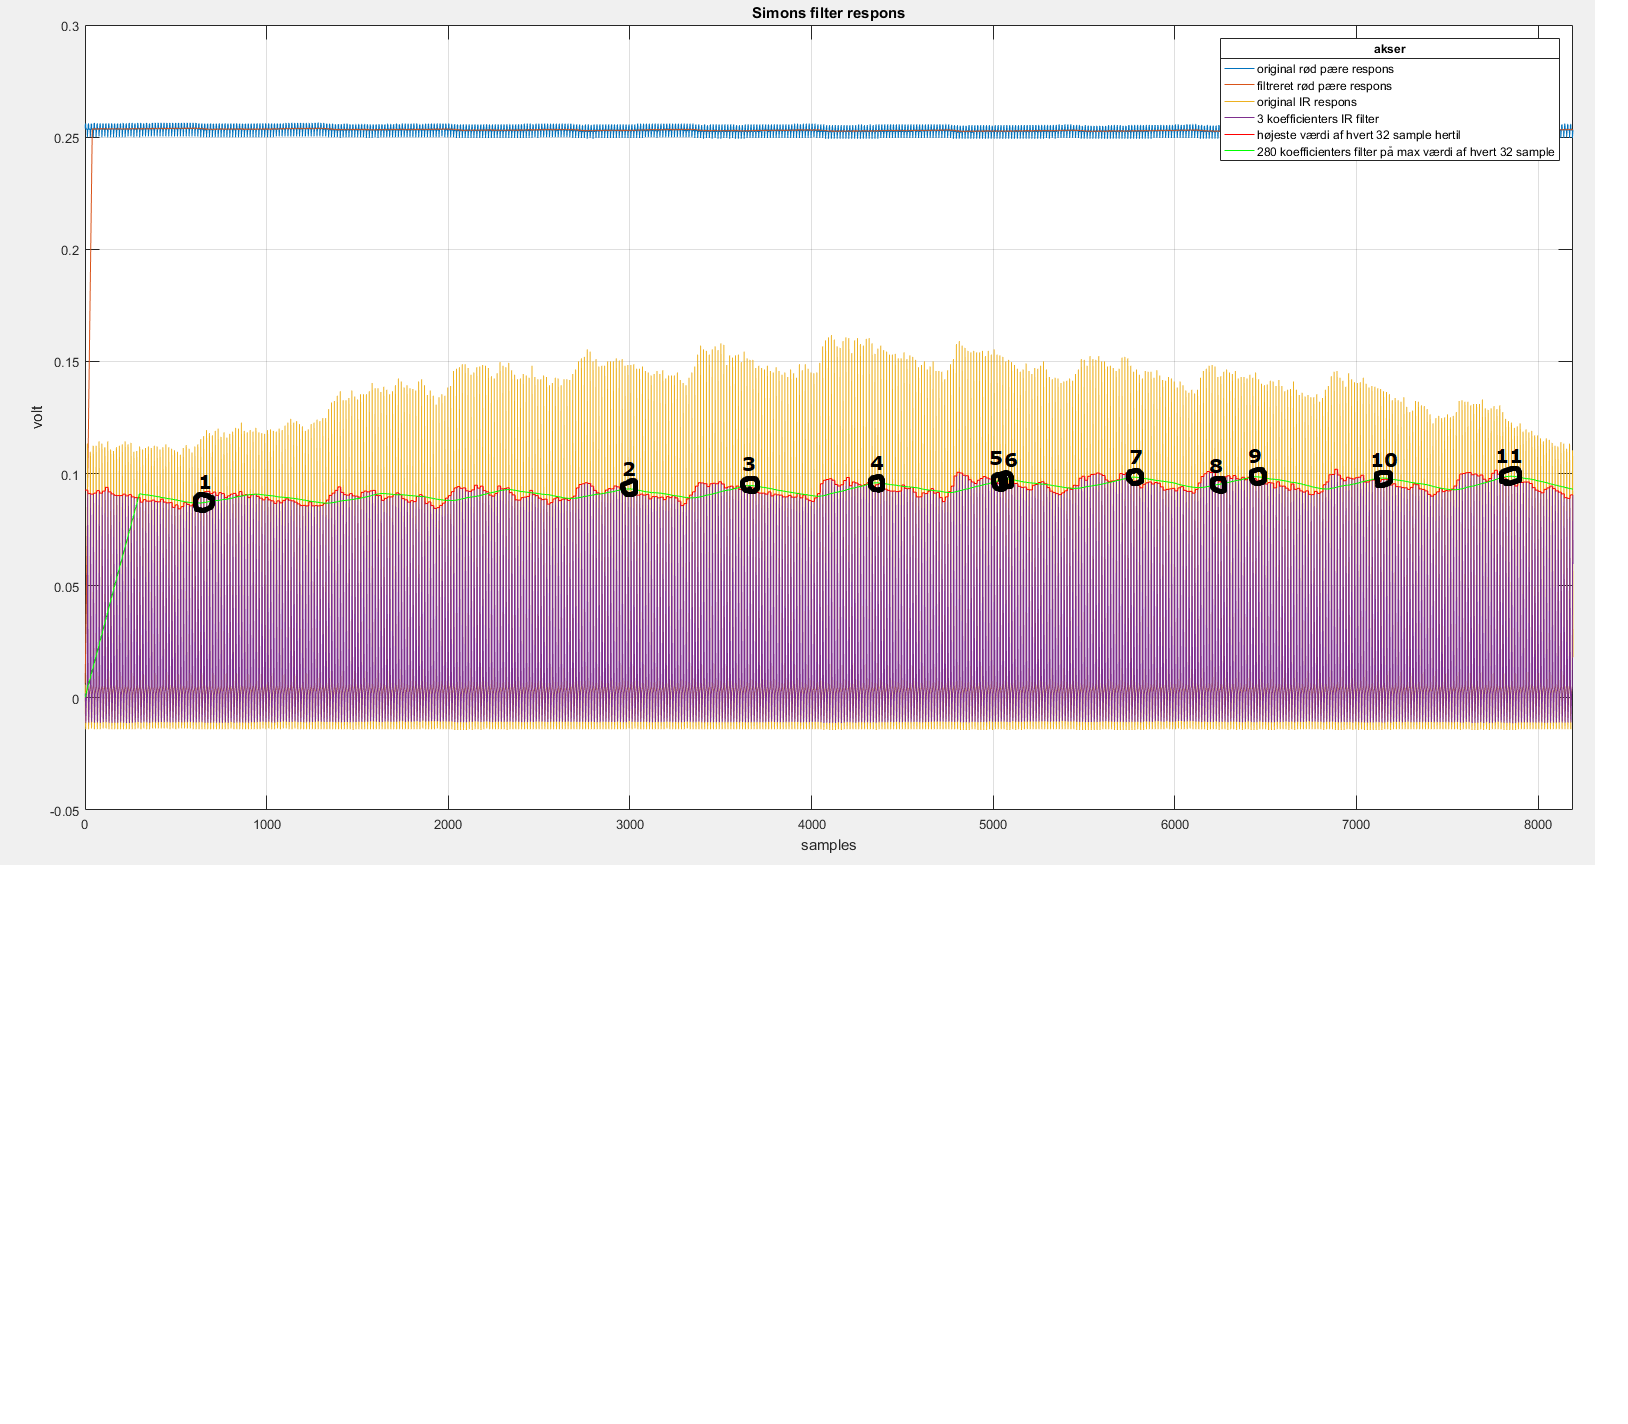
\includegraphics[width=0.7\textwidth]{punkter.png}
  \caption{Højderygge markeret}
  \label{fig:punkter}
\end{figure}

Den første højderyg er hvorfra filtereret er aktivt. Tiden, $\Delta t$, mellem den anden højderyg (den første højderyg som følge af et pulsslag), $p_x(2)$, og sidste højderyg, $p_x(12)$ er:
\begin{equation}
  \label{eq:5}
  \Delta t=\frac{p_x(12)-p_x(1)}{800Hz}=9,04s
\end{equation}

Pulsfrekvensen, $f_{puls}$, kan udregnes som

\begin{equation}
  \label{eq:6}
  f_{puls}=\frac{60}{\Delta t}\cdot 12=79,4\mathrm{\ slag\ pr.\ minut}
\end{equation}

Dette svarer til følgende matlab-kode:
\begin{lstlisting}[language=Matlab,basicstyle=\tiny]
  pulsfr=(60/((p_x(length(p_x))-p_x(1))/800))*puls;
\end{lstlisting}

Pulsfrekvensen findes altså at være 79.

\section{Konklusion}
\label{sec:konklusion}

Rapporten har vist hvordan digitalsignal analyse med bl.a. midlingsfiltrering kan udregne pulsfrekvens og iltprocent fra målinger af gennemlysning af rødt og infrarødt lys i en finger. Dette er blevet sammenholdt med målinger med et konventionelt pulsoximeter.
Der er vist en pæn overensstemmelse og samtidig nytten af dataoprensning med midlingsfiltre.
\clearpage
\appendix
% iso-latin-1-unix
% utf-8-dos

\section{Matlab-kode}
\label{sec:appendix-vhdl-koden}
\lstinputlisting[basicstyle=\footnotesize\ttfamily,language=Matlab,basicstyle=\tiny,numbers=left]{d:/Projekter/Matematik/int_dig_ana/opgaver/Caseprojekter/case_4/case4.m}

\end{document}
